\documentclass[portrait]{a0poster}


\usepackage[latin1]{inputenc}
\usepackage{amsfonts}
\usepackage{amsmath}
\usepackage[english]{babel}
\usepackage{fontenc}
\usepackage{graphicx}
\graphicspath{{images/}}

\usepackage[absolute]{textpos}

\usepackage{color}
\usepackage{tikz}
\usetikzlibrary{shapes,snakes, fadings}

\usepackage[pdftex]{hyperref}

% \usepackage{background}
\usepackage{multicol}


% \backgroundsetup{
% scale=0.5,
% angle=0,
% opacity=1,
% contents={\begin{tikzpicture}[remember picture,overlay]
%  \path [top color = tardisblue, middle color = tardisblue!30, bottom color = white] (current page.south west)rectangle (current page.north east);
% \end{tikzpicture}}
% }


%redefinir l'espacement entre les lignes
\renewcommand{\baselinestretch}{1.4}


% \definecolor{tardisblue}{rgb}{16,35,114}
\definecolor{tardisblue}{HTML}{102372}
\def\d{\textrm{d}}


% How to use textblock :
%\begin{textblock}{size}[anchorage: relative_x,relative_y](x,y)
%\end{textblock}

%A0 : 841mm x 1189mm


% \tikzfading[name=fading_up_down,
%   left color=red!0, right color=red!100]


% \pagecolor{tardisblue!10}

\begin{document}

\setlength{\TPHorizModule}{1cm} % �chelle horizontale
\setlength{\TPVertModule}{\TPHorizModule} % �chelle verticale identique � l'horizontale


 % Define box and box title style
  
\tikzstyle{background_box} = [top color=tardisblue!70,
  bottom color=tardisblue!40,rectangle, rounded corners, inner sep=10pt, inner ysep=20pt]  
    
\tikzstyle{boite1bis} = [draw=tardisblue, fill=white, line width=2mm,
    rectangle, rounded corners, inner sep=10pt, inner ysep=20pt]

\tikzstyle{boite2bis} = [draw=red, fill=white, line width=2mm,
    rectangle, rounded corners, inner sep=10pt, inner ysep=20pt]

\tikzstyle{titre1} =[fill=red!40, text=black, rounded corners]

\tikzstyle{boite2} = [draw=red, fill=green!10, very thick,
    rectangle, rounded corners, inner sep=10pt, inner ysep=20pt]



\tikzstyle{fondblanc}=[fill=white, inner sep=0pt, inner ysep=0pt]

% \tikzstyle{poster_background}=[fill=red, fading=fading_up_down]




%--------------------------------------
%BACKGROUND
%--------------------------------------

\begin{textblock}{85.2}[0,0](0,0.25)
\begin{tikzpicture}
\node[background_box](box){
     \begin{minipage}{1.00\linewidth}
     \phantom{a} \hspace{3cm} \phantom{b}\\
     
\vspace{112cm}

\phantom{b}
     \end{minipage}
  };
\end{tikzpicture}
\end{textblock}



%--------------------------------------
%**************TITRE******************
%--------------------------------------



\begin{textblock}{83}(1,1)
 \begin{tikzpicture}

\node [boite1bis] (box){%
    \begin{minipage}{1.00\textwidth}
	  \begin{center}
	  {\veryHuge Detecting Additional Polarization Modes with eLISA}\\
	  \vspace{2cm}
	  {\huge L. Philippoz, P. Jetzer}\\
	  \end{center}
\end{minipage}
};

\end{tikzpicture}%
\end{textblock}



\begin{textblock}{9}[1,0](81.5,2.5)
\begin{tikzpicture}
\node[fondblanc](box){
  
\includegraphics[height=4.0cm]{uzh_logo_e_pos_a0.pdf}
  };
\end{tikzpicture}
\end{textblock}


% \begin{textblock}{9}[0,0](2,1.8)
% \begin{tikzpicture}
% \node[fondblanc](box){
%   
\includegraphics[height=4.8cm]{tardis_logo.png}
%   };
% \end{tikzpicture}
% \end{textblock}
 



%--------------------------------------
%************** SUMMARY **************
%--------------------------------------

 
 \begin{textblock}{60}[0.5,0](43,10)
 \begin{tikzpicture}
\node [boite1bis] (box){%
    \begin{minipage}{1.00\textwidth}
    \vspace{1.5cm}
    {\large Within the frame of Einstein's General Relativity, gravitational waves are expected to possess two tensorial polarizations, namely the 
well-known $h_+$ and $h_\times$ modes. Other metric theories of gravity however allow the existence of additional modes (two vector and/or 
two scalar modes), and the (non-)observation of those additional polarizations could put constraints on the validity of all existing theories, 
which would consequently provide a further test for General Relativity.}\\

{\large In its 2-arm-planned-configuration, eLISA only consists of one detector orbiting around the Sun, and we therefore investigate if there is a 
possibility to still detect and separate additional modes of a given gravitational wave signal.
}\\
    \end{minipage}
};

\node[titre1, right=20pt] at (box.north west) {{\LARGE Summary}};
\end{tikzpicture}%
\end{textblock}






%--------------------------------------
%************** OBEN-LINKS **************
%--------------------------------------

 \begin{textblock}{40}(1,28)
 \begin{tikzpicture}
\node [boite1bis] (box){%
\begin{minipage}{1.00\textwidth}
    \vspace{1.5cm}
    {\large Perturbed metric corresponding to a propagating gravitational wave:
    \begin{equation*}
     h_{ij}(\omega t - \mathbf{k}\cdot\mathbf{x}) = \sum_A h_A(\omega t - \mathbf{k}\cdot\mathbf{x}) e_{ij}^A
    \end{equation*}
    with $A=\times, +, b, l, x,y$ the six possible polarization modes and the following tensors (tensor, scalar and vector modes)\\}    
    \begin{minipage}{0.5\linewidth}
    \begin{eqnarray*}
     e_{ij}^+=\left(\begin{array}{ccc}1&0&0\\0&-1&0\\0&0&0\end{array}\right) && 
e_{ij}^\times\left(\begin{array}{ccc}0&1&0\\1&0&0\\0&0&0\end{array}\right)\\ \phantom{A}&&\\\phantom{a}&&\\
     e_{ij}^b=\left(\begin{array}{ccc}1&0&0\\0&1&0\\0&0&0\end{array}\right) && 
e_{ij}^l\left(\begin{array}{ccc}0&0&0\\0&0&0\\0&0&1\end{array}\right)\\ \phantom{A}&&\\\phantom{a}&&\\
     e_{ij}^x=\left(\begin{array}{ccc}0&0&1\\0&0&0\\1&0&0\end{array}\right) && 
e_{ij}^y\left(\begin{array}{ccc}0&0&0\\0&0&1\\0&1&0\end{array}\right)
    \end{eqnarray*}
     \end{minipage}
     \hfill
     \begin{minipage}{0.5\linewidth}
     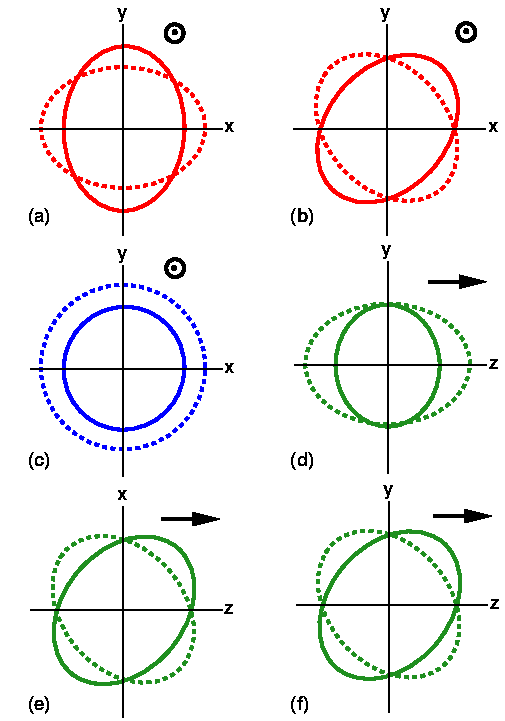
\includegraphics[width=15cm]{polarization_will_review.pdf}
     \end{minipage}
%     {\large Polarization + agencement ($\sim$ Gitter), eLISA + $\mathbf{x}(t)$, etc. (sch\'ema)}
\end{minipage}
};

\node[titre1, right=20pt] at (box.north west) {{\LARGE Polarization modes}};
\end{tikzpicture}%
\end{textblock}


 
 
 
%--------------------------------------
%************ OBEN-RECHTS **************
%--------------------------------------

 \begin{textblock}{40}[0,0](1,64)
 \begin{tikzpicture}
\node [boite1bis] (box){%
  
    \begin{minipage}{1.00\textwidth}
    \vspace{1.5cm}
    {\large %evt d\'efinir la base tensorielle
    \begin{itemize}
    \item GW stochastic background in the low frequency limit
    \begin{equation*}
     h(t, \mathbf{x}) = \sum_{A} \int_{S^2} \d \boldsymbol{\hat\Omega} \int_{-\infty}^\infty \d f \ \tilde{h}_A(f, \boldsymbol{\hat\Omega}) e^{2\pi i 
f (t-\boldsymbol{\hat\Omega} 
\mathbf{x} /c)} F_A(\boldsymbol{\hat\Omega})
    \end{equation*}
    
    with $A=+, \times, x, y, b, l$ all possible polarizations, $F_A$ the antenna pattern function.
   
   \item Overlap reduction function (how much degree of correlation is preserved between detectors)
    \begin{equation*}
     \gamma_{IJ}^M (f) = \frac{1}{\sin^2 \chi} \left( \rho^M_1 (\alpha) D_I^{ij} D_{ij}^J + \rho_2^M (\alpha) D_{I,k}^i D_J^{kj} \hat{d}_i 
\hat{d}_j + \rho_3^M(\alpha) D_I^{ij} D_J^{kl} \hat{d}_i \hat{d}_j \hat{d}_k \hat{d}_l \right)
    \end{equation*}
    
    {\small  with $\rho_i^M = f(j_0(\alpha), j_2(\alpha), j_4(\alpha))$, $\displaystyle \hat{d}_i = \frac{\mathbf{x}}{\left| \mathbf{x} 
\right|}$, $\displaystyle \alpha=\frac{2\pi f \left| \mathbf{x} \right|}{c}$, $M=T,V,S$}
   \item GW background energy density
   $\Omega_\text{gw}^T = \Omega_\text{gw}^+ + \Omega_\text{gw}^\times$ (similar for $\Omega_\text{gw}^V$ and $\Omega_\text{gw}^S$), 
   related to the one-sided power spectral density $S(\left|f\right|) \propto \langle \tilde{h}_A^* (f, \boldsymbol{\hat\Omega}) \tilde{h}_{A'} 
(f',\boldsymbol{\hat\Omega'})\rangle$ by $\Omega_\text{gw}^M(f) \propto f^3 S_h^A (f)$
   \item The tensor, vector and scalar modes can then be separately detected via
   \begin{equation*}
    SNR^M \propto \int_0^\infty \d f \left[ \frac{(\Omega_\text{gw}^M (f))^2 \det \mathbf{F}(f)}{f^6 \mathcal{F}_M(f)} \right]^{(1/2)}
   \end{equation*}
   {\small where the elements of the $(3\times3)$-matrix $\mathbf{F}$ are given by $\displaystyle F_{MM'} = \sum_{\text{det pairs}} \d t 
\frac{\gamma_{IJ}^M (t,f) \gamma_i^{M'}(t,f)}{P_I(f)P_J(f)}$}\\
  \item[$\Rightarrow$] Valid for a network of independant detectors in space (3 LISA-like detectors would be sufficient), in the low frequency limit, 
and for a full polarized GWB
  \item[$\Rightarrow$] ``Static'' system (the relative position of the detectors in the network doesn't change)

   \end{itemize}
       }
    \end{minipage}

};


\node[titre1, right=20pt] at (box.north west) {{\LARGE Stochastic GW background : network of detectors [1]}};
\end{tikzpicture}%
\end{textblock}



 \begin{textblock}{40}[1,0](84,64)
 \begin{tikzpicture}
\node [boite1bis] (box){%
  
    \begin{minipage}{1.00\textwidth}
    \vspace{1.5cm}
    {\large
    \begin{itemize}
     \item If the output data of the single detector is written as $h(t)+n(t)$, with $n(t)$ the noise, the autocorrelation of the signal reads
     \begin{equation*}
      \langle \tilde{h}(f) \tilde{h}^*(f')\rangle = \frac{1}{2} \delta(f-f') S_h(\left| f\right|)
     \end{equation*}
    {\small with $S_h(\left| f \right|)$ the one-sided power spectral density; one can define $S_n$ in a similar way for the noise.}
    \item The maximum SNR given by this process is
    \begin{equation*}
     SNR^2 = \frac{T}{2} \int_{-\infty}^\infty \d f \ \frac{S_h(\left| f \right|)^2}{\left[ S_h(\left| f \right|)+ S_n(\left| f \right|)\right]^2}
    \end{equation*}
    \item[$\Rightarrow$] Also valid in the high-frequency limit, for a single detector, but for an unpolarized GWB
    \end{itemize}

    }
    \end{minipage}

};


\node[titre1, right=20pt] at (box.north west) {{\LARGE Stochastic GW background : single detector [5]}};
\end{tikzpicture}%
\end{textblock}






%--------------------------------------
%************ UNTEN-LINKS *************
%--------------------------------------



\begin{textblock}{40}[1,0](84,28)
 \begin{tikzpicture}
\node [boite1bis] (box){%

    \begin{minipage}{1.00\textwidth}
    \vspace{1.5cm}
    \begin{minipage}{0.5\linewidth}
    {\large \begin{itemize}
	     \item Time-delay interferometric combinations,\\ 2-arm configuration (4 beams)
             \item Noise power spectrum : $S_X(f)$
             \item Root-mean squared GW response : $X_\text{RMS}(f)$
             \item Sensitivity : $\text{SNR}\cdot\sqrt{S_X(f) B}/X_\text{RMS}(f)$\\
             {\normalsize $B$ : 1 cycle/year, SNR=5}
            \end{itemize}
    }
   \end{minipage}
   \hfill
   \begin{minipage}{0.5\linewidth}
    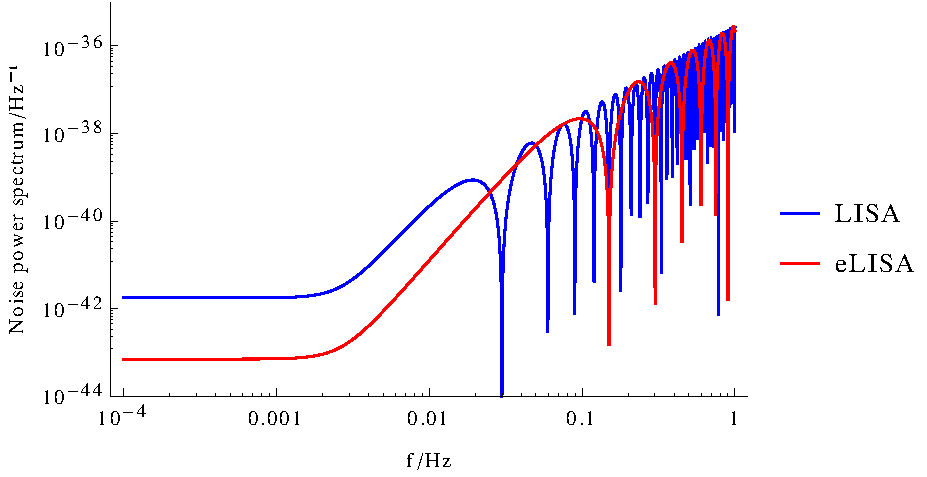
\includegraphics[height=10cm]{noise_power_spectrum}
   \end{minipage}
    
    \vspace{1.4cm}
   
   
   \begin{minipage}{0.5\linewidth}
    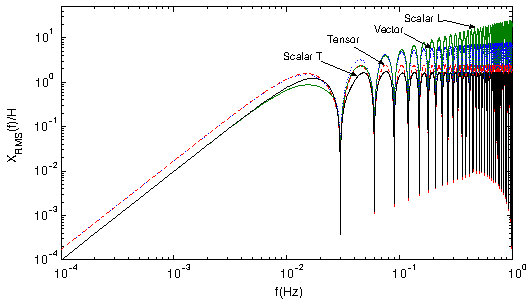
\includegraphics[height=10cm]{rootmeansquare_response}
   \end{minipage}
   \hfill
      \begin{minipage}{0.5\linewidth}
    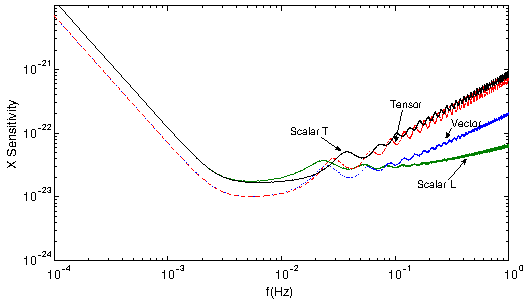
\includegraphics[height=10cm]{sensitivity}
       \end{minipage}

   
   {\large
   \begin{itemize}
   \item Similar behaviour between LISA and eLISA in the high-frequency regime (where they are more sensitive to (longitudinal) scalar modes)
   \item $X_\text{RMS}(f)$ and the sensitivity are given for LISA (similar results expected with shorter arms; to be confirmed)
   \end{itemize}
   }
%    \end{minipage}
%    \hfill
%       \begin{minipage}{0.4\linewidth}
%    \end{minipage}
{\large
%  Is it the case for 1 eLISA over time ? The noise spectrum should remain the same ?
}


    \end{minipage}

};

\node[titre1, right=20pt] at (box.north west) {{\LARGE Sensitivity to additional modes}};
\end{tikzpicture}%
\end{textblock}




%--------------------------------------
%********** UNTEN RECHTS ***********
%--------------------------------------
% 
%   \begin{textblock}{40}[1,0](84,55)
%   \begin{tikzpicture}
%  \node [boite1bis] (box){%
%    
%      \begin{minipage}{1.00\textwidth}
%      \vspace{1.5cm}
%      {\large
%      %Energy density vs f, for each mode
%      Future prospects/Conclusion:
%      \begin{itemize}
%       \item Time dependance
%       \item Sensitivity
%       \item Comparison 2/3
%      \end{itemize}
%  
%      \vspace{5cm}
%      
%      RESULT
%      }
%      \end{minipage}
%  
%  };
%  
%  
%  \node[titre1, right=20pt] at (box.north west) {{\LARGE RESULT}};
%  \end{tikzpicture}%
%  \end{textblock}
% 





%--------------------------------------
%**************CONCLUSION**************
%--------------------------------------
%  
  \begin{textblock}{40}[1,0](84,87)
  \begin{tikzpicture}
 \node [boite1bis] (box){%
     \begin{minipage}{1.00\textwidth}
     \vspace{1.5cm}
     {\large
     \begin{itemize}
      \item Cross-correlating the TDI combinations of a LISA-like single detector also correlates the noise
      \item The separation of all modes however requires a network of detectors
      \item Work in progress
      \begin{itemize}
      \item Letting eLISA evolve on its orbit and correlating the signals at different time
      \item Correlating eLISA signal with future earth-based detectors around 1Hz
      \end{itemize}
     \end{itemize}
}
     \end{minipage}
 };
 
 \node[titre1, right=20pt] at (box.north west) {{\LARGE Possible solutions for eLISA}};
 \end{tikzpicture}%
 \end{textblock}



%--------------------------------------
%************** BIBLIO ****************
%--------------------------------------


  \begin{textblock}{80}[0.5,0.5](42.5,110)
 \begin{tikzpicture}
\node [boite2bis] (box){%
    \begin{minipage}{1.00\textwidth}
    \vspace{1.5cm}
    {\large 
    \begin{multicols}{2}
    \begin{itemize}
             \item[[1\!]] Nishizawa A., Taruya A., Kawamura S., Phys. Rev. D \textbf{81}, 104043 (2010)
             \item[[2\!]] Nishizawa A. et al., Phys. Rev. D \textbf{79}, 082002 (2009)
             \item[[3\!]] Seto N., Phys. Rev. L \textbf{97}, 151101 (2006)
             \item[[4\!]] Seto N., Taruya A., Phys. Rev. D \textbf{77}, 103001 (2008)
             \item[[5\!]] Tinto M., Alves M.E., Phys. Rev. D \textbf{82}, 122003 (2010)
             \item[[6\!]] Estabrook F.B., Tinto M., Armstrong J.W., Phys. Rev. D \textbf{62}, 042002 (2000)
             \item[[7\!]] Tinto M., Armstrong J.W., arXiv:1205.4620v1 [gr-qc]
             \item[[8\!]] Will C., Living Rev Relativity \textbf{9}, (2006), 3.% [Online Article]: cited [17.06.2013]
            \end{itemize}
    \end{multicols}
    %\begin{thebibliography}{99}
            %\bibitem{knoll}Knoll F.G., \emph{Radiation Detection and Measurement}, John Wiley \& Sons, 1999
	    %\bibitem{notice}Bertolloto D., Epiney A., Girardin G., \emph{D�tection et contr�le du flux neutronique}, EPFL, 2007
            %\end{thebibliography}
}
    \end{minipage}
};

\node[titre1, right=20pt] at (box.north west) {{\LARGE References}};
\end{tikzpicture}%
\end{textblock}




\end{document}
